% Shared content of the PlantIQ paper. Edit THIS file; main.tex (two columns, IEEE conference) and
% main_onecol.tex (one column) both \input it, so the two PDFs always have identical content.
\IEEEoverridecommandlockouts
\usepackage{cite}
\usepackage{amsmath,amssymb,amsfonts}
\usepackage{algorithm}
\usepackage{algorithmic}
\usepackage{graphicx}
\usepackage{textcomp}
\usepackage[T1]{fontenc}
\usepackage{newtxtext} % Times text, as in the IEEE template output
\usepackage{xcolor}
\usepackage{booktabs}
\usepackage{multirow}
\usepackage{makecell}
\usepackage{array}
\usepackage{url}
\usepackage{tikz}
% width of single-column figures; main_onecol.tex sets it smaller before \input-ing this file
\providecommand{\plantiqfigw}{\columnwidth}
\usetikzlibrary{arrows.meta,positioning,fit,backgrounds,calc,shapes.geometric}
\def\BibTeX{{\rm B\kern-.05em{\sc i\kern-.025em b}\kern-.08em
    T\kern-.1667em\lower.7ex\hbox{E}\kern-.125emX}}

% ---------------------------------------------------------------------------
% DRAFT MARKERS — remove both macros' colour before submission.
%   \mock{...}  : MOCK comparison value (placeholder until the experiment is run)
%   \tbd{...}   : fact the team must fill in from its own records (e.g. training run)
% ---------------------------------------------------------------------------
\newcommand{\mock}[1]{\textcolor{red}{#1}}
\newcommand{\tbd}[1]{\textcolor{blue}{[#1]}}
\newcommand{\yes}{\checkmark}
\newcommand{\no}{$\times$}
\newcommand{\part}{$\sim$}

\tikzset{
  box/.style={draw=black!70, rounded corners=2pt, align=center, font=\scriptsize, inner sep=3pt, fill=white},
  mod/.style={box, fill=blue!6, minimum width=2.45cm, minimum height=0.95cm},
  ext/.style={box, fill=black!4, dashed},
  arr/.style={-{Stealth[length=4pt]}, black!75, line width=0.5pt},
  grp/.style={draw=black!35, rounded corners=3pt, inner sep=5pt},
  grplabel/.style={font=\scriptsize\bfseries, black!70},
}

\begin{document}

% IEEEtran numbers references in order of first citation. These two are registered first so that the
% coffee CNN paper is [1] and the coffee RAG paper is [2]; all other references follow in citation order.
\nocite{anudeep2024cnn,selvakumar2024rag}

\title{PlantIQ: A Multimodal, Retrieval-Grounded Decision-Support Platform for Smallholder Coffee Growers in Karnataka
\thanks{\textcolor{red}{DRAFT. Values printed in red and figures stamped ``MOCK DATA'' are placeholders for comparison
experiments that have not yet been run; values in blue brackets must be filled in by the authors. All other numbers are
measurements taken from the implemented system.}}
}

% Authors are set as an explicit 2 x 2 table with two equal-width columns, so both rows line up.
% (IEEEtran's \and centres each row by its own widest line, which misaligned the "AI & ML" row.)
% Styling matches IEEEauthorblockN/A: name in normal size, affiliation lines in italics.
\newcommand{\authorcell}[3]{%
  \begin{tabular}[t]{@{}c@{}}
    {\large #1}\\[0.4ex]
    \textit{#2}\\
    \textit{PES University}\\
    Bengaluru, India\\
    #3
  \end{tabular}}

\author{%
\begin{tabular}{@{}p{0.5\textwidth}@{}p{0.5\textwidth}@{}}
\centering\authorcell{Jeel Nada}{Dept. of Computer Science and Engineering}{PES2UG23CS357 \tbd{email}} &
\centering\arraybackslash\authorcell{Nidhi N Udupa}{Dept. of Computer Science and Engineering}{PES2UG23CS384 \tbd{email}} \\
\addlinespace[3ex]
\centering\authorcell{Mohammed Ayaan}{Dept. of Computer Science and Engineering (AI \& ML)}{PES2UG23AM058 \tbd{email}} &
\centering\arraybackslash\authorcell{Prof. Deepti C.}{Dept. of Computer Science and Engineering}{\tbd{email}} \\
\end{tabular}}

\maketitle

\begin{abstract}
Coffee growers in the Chikkamagaluru, Kodagu and Hassan districts of Karnataka face three recurring problems: foliar
diseases that spread quickly during the monsoon, treatment advice that is generic, English-only and blind to the day's
weather, and weak access to buyers for small lots. This paper presents PlantIQ, an Android and web platform backed by a
self-hostable server, organised as four modules. Module 1 diagnoses a single leaf photograph into leaf rust, Cercospora
leaf spot, Phoma leaf spot, leaf miner or healthy with a transfer-learned ResNet-50 and a confidence gate. Module 2
produces a treatment plan grounded in Central Coffee Research Institute extension documents and research literature
through a hybrid retriever that fuses multilingual dense search with BM25 by reciprocal rank fusion, reranks with a
cross-encoder and removes redundancy with maximal marginal relevance; the plan is conditioned on live weather at the
estate, a rule-based fungal infection risk level and a three-day spray window, and every dose in the generated text is
audited against the retrieved passages. Module 3 is a conversational assistant for English and Kannada with
conversation memory, photo and past-scan hand-off, weather-intent detection and on-device speech recognition for
Kannada and Indian English. Module 4 is a marketplace that normalises quantities and prices to kilograms and rupees per
kilogram and ranks lots by great-circle distance. On the development hardware, leaf inference takes 5.3 ms on a laptop
GPU, hybrid retrieval about 0.4 s and a complete advisory about 6 s, dominated by language-model generation.
We show that the public JMuBEN coffee-leaf dataset, whose 58,549 images derive from only 861 distinct leaf
patches, leaks almost every test image into training under a random split, and evaluate with leak-free group-aware
five-fold cross-validation: the PlantIQ classifier reaches a macro-F1 of 0.970, while re-implemented GoogLeNet and
YOLOv8 baselines from prior coffee work reach 0.988 and 0.985 with a quarter of the parameters.
\mock{The retrieval and generation comparison of Modules 2 and 3 is in progress.}
\end{abstract}

\begin{IEEEkeywords}
coffee leaf disease, ResNet-50, retrieval-augmented generation, hybrid retrieval, agricultural advisory,
Kannada speech recognition, decision support, digital agriculture marketplace
\end{IEEEkeywords}

% =========================================================================================
\section{Introduction}
% =========================================================================================
Karnataka produces most of India's coffee, much of it on small holdings in the Western Ghats districts of
Chikkamagaluru, Kodagu and Hassan. Coffee leaf rust (\textit{Hemileia vastatrix}), Cercospora leaf spot
(\textit{Cercospora coffeicola}), Phoma leaf spot (\textit{Phoma costarricensis}) and the coffee leaf miner
(\textit{Leucoptera coffeella}) are favoured by the humid monsoon, and the time between infection and visible damage
across a block is short compared with the interval between visits by extension staff. The disease is only half of the
decision: whether and when to spray also depends on the weather, because rain shortly after a fungicide application
washes it off, while sustained high humidity at moderate temperatures favours fungal infection. Elevation and rainfall
are also known to shape coffee growth and yield in these districts~\cite{patil2022elevation}. Printed extension material
does not adapt to the conditions of a given day and is largely in English, whereas many growers are most comfortable in
Kannada.

Prior coffee-specific work has addressed parts of this problem in isolation. Image classifiers report high accuracy on
curated datasets~\cite{anudeep2024cnn}; detection combined with retrieval-augmented generation (RAG) has been proposed
to reduce hallucination in remediation advice~\cite{selvakumar2024rag}; and general-purpose agricultural chatbots have
been deployed at scale~\cite{singh2024farmerchat}. A recent survey of multi-modal large language models (LLMs) in
agriculture identifies the integration of visual, linguistic and environmental signals as an open
challenge~\cite{sapkota2024mmllm}. To our knowledge, none of the cited systems combines leaf diagnosis, document-grounded
and weather-conditioned advice, a Kannada voice interface and a market channel in a single deployable application.

This paper describes PlantIQ, an implemented system that does so. Its contributions are:
\begin{enumerate}
\item A \textbf{confidence-gated diagnosis pipeline} (Module 1) that wraps a five-class ResNet-50 with input
sanitisation, per-user result caching and an explicit ``blended'' state that is raised when either the image model or
the retrieved evidence is weak, instead of silently returning a low-confidence label.
\item A \textbf{hybrid, hardware-aware RAG advisory} (Module 2) combining multilingual dense retrieval, BM25, reciprocal
rank fusion, a disease-topic filter, cross-encoder reranking and maximal marginal relevance, conditioned on live
microclimate, a fungal infection risk rule and a three-day spray window, with a post-generation dose audit.
\item A \textbf{multilingual, multimodal chatbot} (Module 3) with an LLM-based language router and heuristic fallback,
image and past-scan hand-off, weather-intent detection and a local-first speech-recognition cascade for Kannada and
Indian English.
\item A \textbf{market-discovery module} (Module 4) that normalises heterogeneous trade units to kilograms and
rupees per kilogram and ranks lots by Haversine distance, with owner-only editing and abuse reporting.
\item An \textbf{evaluation protocol} for comparing each module with re-implemented methods from the coffee-specific
literature (Section~VIII), together with system-level measurements of the implementation.
\end{enumerate}

The remainder of the paper is organised as follows. Section~II reviews related work. Section~III gives the system
architecture. Sections~IV--VII describe the four modules. Section~VIII presents the implementation and evaluation setup,
Section~IX the results, Section~X limitations, and Section~XI concludes.

% =========================================================================================
\section{Related Work}
% =========================================================================================
\subsection{Coffee Leaf Disease Recognition}
Anudeep K.S.\ \textit{et al.}~\cite{anudeep2024cnn} classify coffee leaves into leaf rust, leaf miner, Cercospora and
healthy classes with a CNN and softmax classifier, using GoogLeNet transfer learning. Images were drawn from
ScienceDirect and Mendeley sources, with roughly 3{,}000 images for training and 800 for testing, plus about 250 field
images collected near Chikkamagaluru for testing. They study 60/40, 70/30 and 80/20 train--test splits and report the
highest accuracy with the 80/20 split. Phoma is not among their classes. Selva Kumar \textit{et al.}~\cite{selvakumar2024rag}
train YOLOv8 for instance segmentation of coffee leaf diseases (Rust, Miner and Phoma) on Kaggle, open-source and field
images, and extract the predicted label from the rendered output with EasyOCR before passing it to the language model.
PlantIQ instead treats diagnosis as single-leaf classification with ResNet-50~\cite{he2016resnet}, covers both Phoma and
Cercospora, which are visually similar spot diseases, and exposes the full class distribution and an uncertainty state to
the downstream modules.

\subsection{Retrieval-Grounded Agricultural Advice}
RAG~\cite{lewis2020rag} conditions generation on retrieved passages to reduce hallucination. Selva Kumar
\textit{et al.}~\cite{selvakumar2024rag} build a LangChain pipeline in which research PDFs are chunked and embedded with
the OpenAI embedding API into a vector store, and GPT-3.5 generates diagnosis and treatment text for the detected label;
their work focuses on the system design and does not use environmental data. Zhao \textit{et al.}~\cite{zhao2024kg}
take a structured route for \textit{Elaeagnus angustifolia} diseases, combining LLMs with an agricultural knowledge
graph, graph neural networks and a graph attention mechanism, and report a precision of 0.94, recall of 0.92 and
accuracy of 0.93. PlantIQ uses unstructured retrieval but replaces a single dense retriever with a hybrid of dense and
lexical search, adds reranking and diversification, injects live weather into the prompt and audits generated doses.

\subsection{Agricultural Conversational Assistants}
Farmer.Chat~\cite{singh2024farmerchat} is a generative-AI assistant deployed over WhatsApp and Telegram in four
countries, supporting six languages, voice notes and images, and evaluated with RAGAS-style~\cite{es2023ragas}
faithfulness, relevance and context-precision metrics as well as latency and user engagement. Sapkota
\textit{et al.}~\cite{sapkota2024mmllm} survey multi-modal LLMs in agriculture and highlight domain-specific data,
integration with existing systems and robust evaluation as open problems. PlantIQ's chatbot is narrower in crop scope
but adds Kannada language routing, a local Kannada speech model, CNN diagnosis of attached photos and hand-off of
earlier scans into the conversation.

\subsection{Environmental Context and Market Access}
Patil \textit{et al.}~\cite{patil2022elevation} report significant correlations between elevation, rainfall and
leaf growth, bean characteristics and yield of arabica and robusta in Karnataka, motivating the use of location-specific
weather and elevation in advice. Santhosha and Umesh~\cite{santhosha2023yield} predict coffee yield from Central Coffee
Research Institute (CCRI) soil and agronomic records with ensemble classifiers, and Xavier
\textit{et al.}~\cite{xavier2023price} forecast commodity prices with a hybrid ARIMAX and particle-swarm-optimised
support vector regression model. These works forecast yield or price; PlantIQ's market module addresses the
complementary problem of making individual lots discoverable to nearby buyers, and is therefore not compared
quantitatively with them.

Table~\ref{tab:related} summarises the functional scope of the systems discussed.

\begin{table}[t]
\caption{Functional scope of related systems (\yes\ present, \part\ partial, \no\ absent, as described in each paper)}
\label{tab:related}
\centering
\scriptsize
\setlength{\tabcolsep}{2.6pt}
\begin{tabular}{@{}lcccccc@{}}
\toprule
System & \makecell{Leaf\\diag.} & \makecell{Grounded\\advice} & \makecell{Live\\weather} & \makecell{Kan-\\nada} & Voice & Market \\
\midrule
Anudeep K.S.~\cite{anudeep2024cnn} & \yes & \no & \no & \no & \no & \no \\
Selva Kumar~\cite{selvakumar2024rag} & \yes & \yes & \no & \no & \no & \no \\
Zhao~\cite{zhao2024kg} & \yes & \part & \no & \no & \no & \no \\
Farmer.Chat~\cite{singh2024farmerchat} & \part & \yes & \yes & \no & \yes & \part \\
\textbf{PlantIQ (this work)} & \yes & \yes & \yes & \yes & \yes & \yes \\
\bottomrule
\end{tabular}
\end{table}

% =========================================================================================
\section{System Architecture}
% =========================================================================================
PlantIQ follows a thin-client design (Fig.~\ref{fig:arch}). The client is a single React~18 and TypeScript application
that is served by the backend as a web app and packaged with Capacitor~7 as an Android APK. All models run on the
server, so inexpensive phones are supported and models can be upgraded without reinstalling the app. The server address
is configurable at run time, so the same APK can connect to a laptop on an estate's Wi-Fi network, a tunnel, or a cloud
virtual machine.

The server is a FastAPI application (Python~3.11) organised in layers: an ASGI security middleware (request
identifiers, security headers including a content security policy, a 15~MB body limit, per-IP rate limiting), routers
under \texttt{/api/v1}, Pydantic~v2 schemas that validate and normalise every request, and services for the CNN,
retriever, LLM client, language router, environment, chat orchestration and speech recognition. Heavy models are
created lazily as process-wide singletons by a registry, which also allows deterministic fakes to be substituted for
testing. Persistence uses SQLAlchemy~2 over PostgreSQL, or SQLite for zero-configuration deployments; media files are
stored on disk and the knowledge index as a FAISS file plus JSON.

Every external dependency has a fallback: Gemini to Groq to an offline guide for generation, GPU to CPU for inference,
the multilingual ``quality'' retrieval models to smaller ``balanced'' models, local to cloud speech recognition, and
PostgreSQL to SQLite. Missing weather is reported as unavailable and never replaced by invented values.

\begin{figure*}[t]
\centering
\begin{tikzpicture}
  % modules, 2 x 2 grid
  \node[mod] (m1) at (0,0) {\textbf{Module 1: CNN}\\ResNet-50, 5 classes\\confidence gate};
  \node[mod, right=9mm of m1] (m2) {\textbf{Module 2: RAG + Env.}\\hybrid retrieval, LLM\\risk, spray window};
  \node[mod, below=7mm of m1] (m3) {\textbf{Module 3: Chatbot}\\router, memory,\\speech-to-text};
  \node[mod, below=7mm of m2] (m4) {\textbf{Module 4: Market}\\unit normalisation,\\Haversine ranking};
  \draw[arr] (m1) -- node[above, font=\tiny]{diagnosis} (m2);
  \draw[arr, dashed] (m3) -- node[left, font=\tiny]{photos} (m1);
  \draw[arr, dashed] (m3.north east) -- node[pos=0.55, right, font=\tiny, xshift=1pt]{retrieval, weather} (m2.south west);
  % gateway and client
  \node[box, left=9mm of $(m1.west)!0.5!(m3.west)$, minimum width=2.2cm, minimum height=2.0cm] (gw)
       {\textbf{FastAPI gateway}\\security headers, CSP\\rate limit, JWT auth\\upload sanitiser\\Pydantic validation};
  \node[box, left=9mm of gw, minimum width=2.1cm, minimum height=2.0cm, fill=green!6] (app)
       {\textbf{PlantIQ app}\\React 18 + TS\\Android APK / web\\English / Kannada\\camera, mic, GPS};
  \draw[arr, <->] (app) -- node[above, font=\tiny]{HTTPS} node[below, font=\tiny]{JSON} (gw);
  % data layer (right of modules, inside the server)
  \node[box, minimum width=2.9cm, right=11mm of m2, yshift=-1mm] (kb) {Knowledge index\\FAISS + JSON, 14 PDFs};
  \node[box, minimum width=2.9cm, below=1.5mm of kb] (db) {PostgreSQL / SQLite\\users, scans, chats, listings};
  \node[box, minimum width=2.9cm, below=1.5mm of db] (fs) {Media store, sanitised JPEGs};
  % external services (row below the server)
  \coordinate (below) at ($(m3.south)!0.5!(m4.south)+(0,-1.45)$);
  \node[ext, anchor=north] (llm) at (below) {Gemini 2.5 Flash $\rightarrow$ Groq gpt-oss-120b};
  \node[ext, left=3mm of llm] (om) {Open-Meteo forecast API};
  \node[ext, right=3mm of llm] (stt) {Cloud speech fallback: whisper-large-v3};
  \begin{scope}[on background layer]
    \node[grp, fit=(m1)(m4), inner sep=7pt] (mods) {};
    \node[grp, fit=(kb)(fs), fill=black!2, inner sep=4pt] (data) {};
    \node[grp, fit=(om)(stt), fill=black!2, inner sep=4pt] (extg) {};
    \node[grp, fit=(gw)(mods)(data), inner sep=8pt, label={[grplabel]above:PlantIQ server (laptop or cloud VM)}] (srv) {};
  \end{scope}
  \node[grplabel, anchor=south] at (data.north) {Data layer};
  \node[grplabel, anchor=north] at (extg.south) {External services};
  \draw[arr] (gw.east) -- (gw.east -| mods.west);
  \draw[arr, <->] (mods.east |- data.west) -- (data.west);
  \draw[arr] (mods.south) -- (mods.south |- extg.north);
\end{tikzpicture}
\caption{PlantIQ system architecture. The mobile client is a thin client; all models run on the self-hostable server.
Module 1 feeds its diagnosis to Module 2; Module 3 reuses Modules 1 and 2 for photos, retrieval and weather.}
\label{fig:arch}
\end{figure*}

% =========================================================================================
\section{Module 1: Leaf Disease Diagnosis}
% =========================================================================================
\subsection{Classes and Data}
The classifier distinguishes the five classes in Table~\ref{tab:classes}. Leaf miner is an insect pest rather than a
pathogen but produces characteristic leaf damage and is therefore included.

Training and evaluation use the public JMuBEN Arabica coffee-leaf dataset~\cite{jepkoech2021jmuben}, photographed on
a plantation in Kirinyaga, Kenya: 58,549 128$\times$128-pixel leaf-patch images (healthy 18,983, leaf miner 16,978, leaf rust 8,336, Cercospora 7,681, Phoma
6,571). An audit with MD5 hashes, a rotation- and flip-invariant perceptual hash and a pixel-difference check shows that
these are only 3,756 byte-unique images derived from 861 distinct leaf patches (nine for the healthy class); 94\% of the
files are byte-identical copies and the rest are rotated, flipped or colour-shifted copies. Under a random file split,
99.96\% of test images have a byte-identical copy in the training set, which explains the near-perfect accuracies that
random splits of this dataset produce. All models in this paper are therefore trained and evaluated on group-aware folds
in which every copy of a patch stays on the same side (Section~\ref{sec:protocol}).

The classifier starts from ImageNet-pre-trained ResNet-50 weights~\cite{deng2009imagenet}. Inputs are resized to
224$\times$224 and augmented with AutoAugment (ImageNet policy). Training uses AdamW (learning rate
$3\times10^{-4}$, weight decay $10^{-4}$), cross-entropy loss, a cosine schedule over at most 25 epochs of 6,000 samples
drawn in proportion to the dataset's copy counts, batch size 64 and mixed precision. The checkpoint with the best
validation macro-F1 (ties broken by the lower validation loss) is kept, with early stopping after eight epochs without
improvement; the validation set is a group-disjoint sixth of each training fold. The integrity of the deployed weights
is verified by a SHA-256 check in the test suite.

\begin{table}[t]
\caption{Diagnosis classes of Module 1}
\label{tab:classes}
\centering
\scriptsize
\begin{tabular}{@{}lll@{}}
\toprule
Class & Causal agent & Type \\
\midrule
Coffee leaf rust & \textit{Hemileia vastatrix} & fungal disease \\
Cercospora leaf spot & \textit{Cercospora coffeicola} & fungal disease \\
Phoma leaf spot & \textit{Phoma costarricensis} & fungal disease \\
Coffee leaf miner & \textit{Leucoptera coffeella} & insect pest \\
Healthy & -- & -- \\
\bottomrule
\end{tabular}
\end{table}

\subsection{Input Sanitisation}
Because the classifier receives untrusted uploads from the public internet, every image first passes a guard that
accepts only JPEG, PNG and WebP identified by their file signature rather than their extension, rejects empty files,
files over 10~MB and images with a side over 4096 pixels (a defence against decompression bombs), applies the EXIF
orientation, removes all metadata including GPS coordinates, and re-encodes the image as a clean JPEG. The same guard is
used by the chatbot and the marketplace.

\subsection{Network}
The image is converted to RGB, resized to $224\times224$, scaled to $[0,1]$ and normalised per channel with the ImageNet
mean $(0.485, 0.456, 0.406)$ and standard deviation $(0.229, 0.224, 0.225)$. The backbone is ResNet-50~\cite{he2016resnet},
whose bottleneck residual blocks ($1\times1$, $3\times3$, $1\times1$ convolutions) learn a residual mapping
\begin{equation}
\mathbf{y} = \mathcal{F}(\mathbf{x}, \{W_i\}) + \mathbf{x},
\end{equation}
so that gradients propagate through the identity shortcut. The four stages contain 3, 4, 6 and 3 blocks and end in
global average pooling to a 2048-dimensional feature vector. The original 1000-way classifier is replaced by a head of
dropout ($p=0.4$) followed by a linear layer $2048\rightarrow5$. The model has 23.5~million parameters.

\subsection{Confidence Gate}
The five logits $z_i$ are converted to probabilities by the softmax
\begin{equation}
p_i = \frac{e^{z_i}}{\sum_{j=1}^{5} e^{z_j}}, \qquad c = 100\cdot\max_i p_i ,
\end{equation}
and the full distribution is returned with the top class and its confidence $c$ (in percent). A result is marked
\emph{blended} when
\begin{equation}
c < \tau_c \;\;\lor\;\; \big(\hat{y} \neq \textit{Healthy} \,\land\, s_{\max} < \tau_r\big),
\label{eq:blend}
\end{equation}
where $\tau_c=75\%$, $s_{\max}$ is the best reranked passage score from Module~2 and $\tau_r=0.60$. Healthy leaves are
exempt from the evidence condition because they require no disease protocol. A blended result is shown to the grower
as ``not fully sure'' and the generation prompt instructs the LLM to name look-alike conditions and to recommend
checking more leaves, so that a low-confidence prediction is never presented as a confirmed diagnosis.

\subsection{Serving}
Weights are loaded with PyTorch's weights-only deserialiser under PyTorch~2.7.1, because versions before 2.6 are
affected by CVE-2025-32434, which allowed code execution while loading a checkpoint even in weights-only mode.
Inference runs in PyTorch's inference mode, under a lock on a single model instance per process, on CUDA when
available. Results are cached under the SHA-256 digest of the image bytes, user identifier,
question and language, so a repeated photo is answered immediately while results are never shared across users.

% =========================================================================================
\section{Module 2: RAG Advisory with Environmental Context}
% =========================================================================================
Fig.~\ref{fig:rag} shows the offline indexing and the online advisory pipeline.

\begin{figure}[t]
\centering
\begin{tikzpicture}[node distance=2.2mm, every node/.style={font=\scriptsize}]
  \node[box, minimum width=3.6cm] (q) {Diagnosis $\hat{y}$, $c$ + question + language};
  \node[box, below=of q, minimum width=3.6cm] (route) {Language routing + intent expansion};
  \node[box, below left=2.6mm and -1.55cm of route, minimum width=1.75cm] (dense) {Dense top-20\\bge-m3 / FAISS};
  \node[box, below right=2.6mm and -1.55cm of route, minimum width=1.75cm] (bm) {BM25 top-20};
  \node[box, below=13mm of route, minimum width=3.6cm] (rrf) {Reciprocal rank fusion ($k=60$)};
  \node[box, below=of rrf, minimum width=3.6cm] (topic) {Disease-topic filter (relaxed if $<3$)};
  \node[box, below=of topic, minimum width=3.6cm] (rr) {Cross-encoder rerank, $\sigma(z)$};
  \node[box, below=of rr, minimum width=3.6cm] (mmr) {MMR ($\lambda=0.75$) $\rightarrow$ top 3};
  \node[box, below=of mmr, minimum width=3.6cm, fill=blue!6] (prompt) {Fenced prompt};
  \node[box, right=4mm of prompt, minimum width=1.7cm, fill=green!6] (env) {Open-Meteo\\risk + spray\\window};
  \node[box, below=of prompt, minimum width=3.6cm] (llm) {Gemini $\rightarrow$ Groq $\rightarrow$ offline guide};
  \node[box, below=of llm, minimum width=3.6cm] (audit) {Dose audit vs.\ passages};
  \node[box, below=of audit, minimum width=3.6cm, fill=blue!6] (out) {Advice + citations + risk + badge};
  \node[box, left=4mm of dense, minimum width=1.45cm, fill=black!4] (idx) {Offline:\\14 PDFs\\$\rightarrow$ 931\\chunks};
  \draw[arr] (q) -- (route);
  \draw[arr] (route) -- (dense); \draw[arr] (route) -- (bm);
  \draw[arr] (dense) -- (rrf); \draw[arr] (bm) -- (rrf);
  \draw[arr] (rrf) -- (topic); \draw[arr] (topic) -- (rr); \draw[arr] (rr) -- (mmr); \draw[arr] (mmr) -- (prompt);
  \draw[arr] (env) -- (prompt);
  \draw[arr] (prompt) -- (llm); \draw[arr] (llm) -- (audit); \draw[arr] (audit) -- (out);
  \draw[arr, dashed] (idx) -- (dense);
\end{tikzpicture}
\caption{Module 2 advisory pipeline: hybrid retrieval over the extension corpus, conditioned on live weather, followed
by generation and a post-generation dose audit.}
\label{fig:rag}
\end{figure}

\subsection{Knowledge Base and Chunking}
The corpus consists of 14 PDF documents: CCRI coffee cultivation material, coffee-disease manuals, and research articles
on leaf rust management, the coffee leaf miner, arthropod pests of arabica, Cercospora, nutrient status, organo-mineral
fertilisation and irrigation. One document is a scanned image without a text layer and contributes almost no text.
Running text is extracted per page and tables are extracted separately as Markdown so that spray schedules and dose
tables remain intact. Lines that are upper-case, numbered, end in a colon in title case, or are short and contain
agronomy keywords start a new section. Sentence splitting protects agronomic abbreviations (e.g.\ \textit{a.i.},
\textit{WP.}, \textit{spp.}) and decimals so that a dose such as 0.5\% is not split. Sections are packed into chunks of
about 225 words with about 38 words of sentence overlap; each chunk is prefixed with its section title and tagged with
one of nine topics (leaf rust, Cercospora, leaf miner, Phoma, anthracnose and black rot, nutrition, pest management,
cultural and shade management, general agronomy) by keyword rules. Repeated running headers are removed. The resulting
index contains 931 chunks. It is stored as a FAISS index, a JSON chunk file and a JSON metadata file recording the
embedding model and dimension; no Python \texttt{pickle} is used, because loading pickled files executes code.

\subsection{Hardware-Aware Model Profiles}
Two retrieval profiles are defined (Table~\ref{tab:profiles}). In automatic mode the server selects the \emph{quality}
profile when a CUDA GPU with at least 6~GB memory is present and falls back to \emph{balanced} otherwise, or if the
quality models fail to load. The index records its embedder and is rebuilt automatically when the profile changes.
Models are stored locally in the safetensors format so that they can be memory-mapped and loaded offline.

\begin{table}[t]
\caption{Retrieval model profiles}
\label{tab:profiles}
\centering
\scriptsize
\setlength{\tabcolsep}{3pt}
\begin{tabular}{@{}lll@{}}
\toprule
Profile & Embedding model & Cross-encoder reranker \\
\midrule
\makecell[l]{Quality\\(GPU $\geq$ 6 GB)} & \makecell[l]{BAAI/bge-m3~\cite{chen2024bgem3}\\1024-d, fp16} & \makecell[l]{BAAI/bge-reranker-\\v2-m3} \\
\addlinespace
\makecell[l]{Balanced\\(CPU)} & \makecell[l]{BAAI/bge-base-en-v1.5\\768-d} & \makecell[l]{cross-encoder/ms-marco-\\MiniLM-L-6-v2} \\
\bottomrule
\end{tabular}
\end{table}

bge-m3 is multilingual, so a Kannada query can be embedded directly against the English corpus; in addition, the query
is routed to English keywords as described in Section~VI.

\subsection{Query Construction}
Two queries are built. The \emph{recall query} concatenates ``coffee'' and the class name, the router's English
rewrite of the grower's question, and intent-specific expansions when the question concerns timing (``spray schedule
calendar pre-monsoon post-monsoon''), dose (``dosage concentration per barrel 200L''), organic control, shade and
pruning, or nutrition; English and Kannada trigger words are recognised. The \emph{rerank query} is a natural-language
question, e.g.\ ``How to manage Coffee Leaf Rust on coffee? \ldots'', because cross-encoders are trained on questions
rather than keyword lists.

\subsection{Hybrid Retrieval}
\textit{Dense retrieval} encodes the recall query with the profile's embedder and performs exact inner-product search in
a FAISS \texttt{IndexFlatIP}~\cite{johnson2021faiss} over L2-normalised vectors, which equals cosine similarity,
\begin{equation}
s_{\mathrm{dense}}(q,d) = \frac{\mathbf{e}_q^{\top}\mathbf{e}_d}{\lVert\mathbf{e}_q\rVert\,\lVert\mathbf{e}_d\rVert}.
\end{equation}
Exact search is used because a scan over 931 vectors is fast; approximate indexes are only needed at much larger scale.
\textit{Sparse retrieval} scores chunks with Okapi BM25~\cite{robertson2009bm25},
\begin{equation}
s_{\mathrm{bm25}}(q,d)=\sum_{t\in q}\mathrm{IDF}(t)\,\frac{f(t,d)\,(k_1+1)}{f(t,d)+k_1\big(1-b+b\,\frac{|d|}{\mathrm{avgdl}}\big)},
\end{equation}
with the library defaults $k_1=1.5$ and $b=0.75$. Dense search captures paraphrase (``orange powder on leaves'' versus
``urediniospores''), whereas BM25 captures exact chemical names, concentrations and pathogen names. Each retriever
returns its top 20 chunks, and the two rankings are fused by reciprocal rank fusion~\cite{cormack2009rrf},
\begin{equation}
\mathrm{RRF}(d)=\sum_{r\in\{\mathrm{dense},\,\mathrm{bm25}\}}\frac{1}{k+\mathrm{rank}_r(d)},\quad k=60,
\end{equation}
where a chunk missing from one list is assigned rank 1000. RRF needs no score calibration between the two retrievers.

\subsection{Topic Filter, Reranking and Diversification}
Chunks whose topic matches the diagnosed class are kept first; if fewer than three remain, the best off-topic chunks are
appended after them. The candidates are scored by a cross-encoder~\cite{nogueira2019rerank} that reads the rerank query
and the passage jointly and outputs a logit $z$, mapped to a bounded relevance score
\begin{equation}
s = \sigma(z) = \frac{1}{1+e^{-z}} .
\end{equation}
Finally, maximal marginal relevance~\cite{carbonell1998mmr} selects three passages that are relevant but not redundant,
\begin{equation}
d^{*}=\arg\max_{d\in C\setminus S}\Big[\lambda\, s(d)-(1-\lambda)\max_{d'\in S}J(d,d')\Big],\quad \lambda=0.75,
\end{equation}
where $S$ is the set already selected and $J$ is the Jaccard similarity of token sets. A least-recently-used cache holds
the last 256 queries. If the reranker cannot be loaded, normalised RRF scores are used instead.

\subsection{Environmental Context}
The location comes from the phone's GPS or from coordinates typed by the grower (a bilingual guide explains how to copy
them from Google Maps). The server queries the Open-Meteo forecast API for current temperature, apparent temperature,
relative humidity, rain, wind speed and elevation, and for a three-day daily forecast of precipitation sum, precipitation
probability and minimum and maximum temperature. Coordinates are mapped to Chikkamagaluru, Kodagu or Hassan by bounding
boxes. Responses are cached for 60~s per coordinate cell of about 100~m; there is one retry on HTTP 429 or 503 and a
6~s timeout. If no coordinates are available or the service fails, the response is explicitly marked unavailable and the
prompt instructs the LLM not to state any numbers. Soil pH is not measured; a constant of 6.2 is shown and labelled as an
estimate.

A rule-based fungal infection risk level is computed from temperature $T$ (\textdegree C), relative humidity $H$ (\%)
and today's rain $R$ (mm):
\begin{equation}
\mathrm{risk}=
\begin{cases}
\text{high}, & H \ge 80 \;\land\; 20 \le T \le 28,\\
\text{moderate}, & H \ge 65 \;\lor\; R > 0,\\
\text{low}, & \text{otherwise}.
\end{cases}
\end{equation}
The interface presents the level with an icon, a text label and a three-segment meter so that colour is never the only
cue. A spray window is recommended by Algorithm~\ref{alg:spray}.

\begin{algorithm}[t]
\caption{Three-day spray window}
\label{alg:spray}
\begin{algorithmic}[1]
\REQUIRE daily forecasts $D_0, D_1, D_2$ with rain probability $P_i$ (\%) and rain total $R_i$ (mm); flag $\mathit{rainingNow}$
\FOR{$i = 0$ \TO $2$}
  \STATE $\mathit{dry} \leftarrow (P_i \text{ unknown} \lor P_i < 40) \land (R_i \text{ unknown} \lor R_i < 2)$
  \IF{$i = 0 \land \mathit{rainingNow}$} \STATE $\mathit{dry} \leftarrow$ false \ENDIF
  \IF{$\mathit{dry}$} \RETURN ``spray on day $i$'' \ENDIF
\ENDFOR
\RETURN ``wait for a dry spell''
\end{algorithmic}
\end{algorithm}

\subsection{Generation}
The prompt has a system instruction defining the role of a coffee agronomist and declaring that text inside
\texttt{<user\_query>} and \texttt{<agronomic\_context>} is data, never instructions; the diagnosis with its confidence;
the weather block (or the explicit ``not available'' notice); the grower's question, cleaned of control characters and
the characters \texttt{<>\{\}[]} and truncated to 500 characters; the three passages with source and page; and output
rules. The rules require Kannada script or simple English, sections titled \emph{Do today}, \emph{Spray},
\emph{Timing} and \emph{Prevent}, doses per 200~L barrel only when they appear in the context (otherwise ``follow the
label''), the next dry window when rain is forecast, a statement of uncertainty when the result is blended, and a final
line naming the documents used.

The LLM chain calls Google Gemini 2.5 Flash at temperature 0.2 with its ``thinking'' budget set to zero and at least 2048
output tokens; in our runs the thinking tokens otherwise consumed the output budget and truncated advisories, and a
response that ends with the \texttt{MAX\_TOKENS} finish reason is treated as a failure. On error or rate limiting the
request falls back to Groq's gpt-oss-120b and, if no provider is reachable, to a built-in bilingual offline card per
class (summary, actions, spray, timing and prevention) followed by excerpts of the retrieved passages. All generated text
passes a secret-redaction filter.

\subsection{Dose Audit}
Generated agronomic advice is risky mainly when it states a wrong quantity. After generation, every number followed by a
unit (\%, kg, g, ml, L, ppm) is extracted, normalised, and searched for in the concatenated retrieved passages
(Algorithm~\ref{alg:audit}). The result is shown as ``Doses checked'' or as ``Check doses before mixing'' with the list
of unverified quantities. The audit is a string-level check and does not establish agronomic correctness; it detects
quantities that are not supported by the evidence.

\begin{algorithm}[t]
\caption{Post-generation dose audit}
\label{alg:audit}
\begin{algorithmic}[1]
\REQUIRE generated text $A$, retrieved passages $P_1..P_3$
\STATE $Q \leftarrow$ unique matches of \texttt{number (\%|kg|g|ml|l|ppm)} in $A$
\STATE $C \leftarrow \mathrm{norm}(P_1 \Vert P_2 \Vert P_3)$ \COMMENT{lower-case, no spaces, unit synonyms unified}
\STATE $U \leftarrow \{\, q \in Q : \mathrm{norm}(q) \notin C \,\}$
\RETURN $(\mathit{verified} = (U=\emptyset),\; Q,\; U)$
\end{algorithmic}
\end{algorithm}

Each result also lists its citations (document, page, section and relevance score), which the app shows under
\emph{Sources}.

% =========================================================================================
\section{Module 3: Multilingual Multimodal Chatbot}
% =========================================================================================
\subsection{Message Pipeline}
For each message the server (i) creates a thread or verifies that the thread belongs to the caller, (ii) loads the last
eight messages as history, (iii) runs Module~1 on an attached photo, either a new upload sanitised as in Section~IV-B
or a photo from the user's scan history after an ownership check, (iv) attaches the metadata of a past scan when the
grower taps ``ask in chat'' on a result, (v) obtains weather from the GPS fix or, if absent, from coordinates parsed out
of the message text (e.g.\ ``13.31, 75.77'' or ``lat: \ldots\ lng: \ldots''), (vi) routes the language, (vii) detects
weather intent, (viii) retrieves three passages with Module~2's retriever unless the message is only a greeting or a
place name, and (ix) generates the reply with the same provider chain. Both messages are stored.

\subsection{Language Router}
A short JSON-mode prompt (temperature 0.1) asks the LLM for the detected language (Kannada or English), an
English search query, whether the message is only a greeting or location, and the target response language. If the LLM
is unavailable or returns invalid JSON, a heuristic router uses the Kannada Unicode block (U+0C80--U+0CFF), greeting
words, and a single capitalised word as a place name. Kannada script in the message, or
the Kannada UI setting, forces a Kannada-script reply.

\subsection{Context Assembly and Safety}
The prompt contains a \texttt{<history>} block of cleaned and length-capped turns, the live estate conditions (or an
explicit statement that the location is missing), the CNN diagnosis of the attached photo, the past-scan record
(disease, confidence, earlier advice and the weather logged at scan time), the retrieved passages and the fenced user
query. Rules forbid the model from claiming it cannot see images when a diagnosis is present and from inventing doses or
weather numbers. Weather questions are detected with English and Kannada keyword lists and receive passages on
microclimate and disease risk together with a rule to report the readings and spray suitability. Without any LLM, the
assistant answers with the offline disease card or a weather summary plus passage excerpts. Threads are private, and
reading, writing or deleting another user's thread returns HTTP 403.

\subsection{Speech Recognition}
The grower chooses the language before recording, because short agricultural utterances are difficult to identify
automatically. Audio recorded with the browser MediaRecorder is checked (container signature, at most 10~MB), decoded by
FFmpeg to 16~kHz mono (truncated to 90~s), and transcribed by a local model: AI4Bharat's IndicConformer-600M multilingual
model for Kannada, and a Whisper-base model~\cite{radford2023whisper} fine-tuned on the Svarah Indian-English accent
dataset for English. If the local model fails or returns empty text, the cascade falls back to Groq's
whisper-large-v3 and then to Gemini audio understanding. The transcript is placed in the input box for the grower to
correct before sending; it is never sent automatically. Local models load on first use and can be disabled
individually by configuration.

% =========================================================================================
\section{Module 4: Market Discovery}
% =========================================================================================
\subsection{Listings and Unit Normalisation}
A listing contains a title, variety (Arabica, Robusta, Liberica or free text), quantity with unit, price with price
unit, farmer name, a ten-digit phone number, address, optional coordinates and up to eight captioned photos uploaded
through the image guard. Growers think in different trade units, so the server, never the client, derives
\begin{equation}
q_{\mathrm{kg}} = q\cdot u(\mathrm{unit}),\qquad p_{\mathrm{kg}} = \frac{p}{u(\mathrm{price\ unit})},
\end{equation}
where $u$ is 1 for kg, $1000n$ for ``$n$ ton'', $100n$ for ``$n$ quintal'', 50 or 60 for 50~kg or 60~kg bags, and $x$
for a custom ``$x$ kg'' unit. For example, 40 bags of 50~kg priced at Rs.~9{,}500 per bag become 2{,}000~kg at
Rs.~190/kg. Totals are bounded to 100{,}000~kg and prices to Rs.~10{,}00{,}000.

\subsection{Search, Filtering and Ranking}
Buyers search case-insensitively over title, variety, address and farmer name with bound SQL parameters, and filter by
variety, minimum lot size and a Rs./kg range on the normalised fields, by maximum distance (15, 30, 60 or 120~km) and
by presence of photos. Distance from the buyer $(\varphi_1,\lambda_1)$ to a lot $(\varphi_2,\lambda_2)$ is the
great-circle distance~\cite{sinnott1984haversine}
\begin{align}
a &= \sin^2\!\tfrac{\Delta\varphi}{2}+\cos\varphi_1\cos\varphi_2\sin^2\!\tfrac{\Delta\lambda}{2},\\
d &= 2R\,\mathrm{atan2}\big(\sqrt{a},\sqrt{1-a}\big),\quad R=6371\ \mathrm{km}.
\end{align}
Results can be sorted by nearest (lots without coordinates last), newest, price ascending or descending, or largest
quantity, and the filter sheet shows the number of matching lots before it is applied.

\subsection{Contact and Moderation}
PlantIQ does not intermediate the sale. Buyers call the farmer (\texttt{tel:}), open WhatsApp with a pre-filled message,
or open a Google Maps route to the lot. Publishing requires sign-in, with a quota of 50 listings per user; only the owner
can edit or delete a listing; any other user can report a listing once, with a reason. Free-text fields are stripped of
angle brackets and all text is rendered escaped.

% =========================================================================================
\section{Implementation and Evaluation Setup}
% =========================================================================================
\subsection{Implementation}
Table~\ref{tab:stack} lists the technology stack. Authentication uses Argon2id password hashing~\cite{biryukov2016argon2}
(time cost 3, 64~MB memory), 15-minute JSON Web Tokens and opaque refresh tokens stored as SHA-256 hashes and rotated on
every use with reuse detection that revokes the whole token family, login lockout and a password policy. Every write
endpoint checks ownership. LLM output is rendered as escaped text rather than raw HTML.

\begin{table}[t]
\caption{Implementation stack}
\label{tab:stack}
\centering
\scriptsize
\setlength{\tabcolsep}{3pt}
\begin{tabular}{@{}p{1.9cm}p{6.0cm}@{}}
\toprule
Layer & Technology \\
\midrule
Client & React 18, TypeScript, Vite; Capacitor 7 Android APK; English/Kannada UI \\
Server & Python 3.11, FastAPI, SQLAlchemy 2, Pydantic v2; PostgreSQL or SQLite \\
Vision & PyTorch 2.7.1 (CUDA 12.1), torchvision ResNet-50 \\
Retrieval & FAISS, rank-bm25, sentence-transformers; bge-m3, bge-reranker-v2-m3 \\
Generation & Gemini 2.5 Flash $\rightarrow$ Groq gpt-oss-120b $\rightarrow$ offline guide, over HTTP \\
Speech & IndicConformer-600M (Kannada), Svarah-tuned Whisper-base (English), Groq whisper-large-v3 \\
Weather & Open-Meteo forecast API \\
Hardware & Laptop, NVIDIA RTX 3070 Laptop GPU (8 GB) \\
\bottomrule
\end{tabular}
\end{table}

\subsection{System Testing}
The implementation is covered by 354 automated tests, all passing at the time of writing (Table~\ref{tab:tests}):
backend unit, integration, functional-journey, security and non-functional tests in pytest; real-model tests that load
the deployed CNN weights and the bge-m3 index; frontend unit and component tests in Vitest; and end-to-end tests in
Playwright at a Pixel~7 viewport. A deterministic fake for each model allows the fast suite to run without GPUs.

\begin{table}[t]
\caption{Automated tests per module (passed / total)}
\label{tab:tests}
\centering
\scriptsize
\setlength{\tabcolsep}{2.4pt}
\begin{tabular}{@{}lcccccc@{}}
\toprule
Module & Unit & Integr. & Security & Real model & Frontend & E2E \\
\midrule
M1 CNN & 16/16 & 11/11 & 8/8 & 3/3 & 2/2 & 1/1 \\
M2 RAG + env. & 42/42 & 1/1 & 1/1 & 1/1 & 5/5 & -- \\
M3 Chatbot & 18/18 & 15/15 & 1/1 & -- & -- & 1/1 \\
M4 Market & 31/31 & 9/9 & 13/13 & -- & 18/18 & 2/2 \\
Platform & 39/39 & 33/33 & 35/35 & -- & 27/27 & 8/8 \\
\bottomrule
\multicolumn{7}{@{}l@{}}{\tiny Functional (3) and non-functional (10) backend tests omitted from columns; total 354/354.}
\end{tabular}
\end{table}

\subsection{Comparative Evaluation Protocol}
\label{sec:protocol}
To compare PlantIQ with prior work on equal terms, the baselines are re-implemented and run on the same data, since the
published numbers were obtained on different datasets and class sets.
\begin{itemize}
\item \textbf{Module 1.} Stratified group five-fold cross-validation over the 3,756 byte-unique JMuBEN images
(861 source patches, seed 42), so that every image is tested exactly once (out-of-fold). The baselines are trained on the
same folds with the same budget of 150,000 training samples: GoogLeNet transfer learning following Anudeep
K.S.\ \textit{et al.}~\cite{anudeep2024cnn} (ImageNet weights, last three layers fine-tuned, Adam, 30 epochs) and YOLOv8
following Selva Kumar \textit{et al.}~\cite{selvakumar2024rag}; because the dataset has class labels but no polygon
masks, the classification variant YOLOv8s-cls replaces their segmentation model. The earlier PlantIQ training recipe
(128-pixel input, linear head, 15 epochs) is retrained on the same folds as a further baseline. Metrics: accuracy,
macro-averaged precision, recall and F1 with 95\% confidence intervals from a bootstrap over source patches, per-class
F1, confusion matrix, expected calibration error and batch-1 latency (median of 200 runs) on the laptop CPU.
\item \textbf{Module 2.} A set of \tbd{N} grower questions per disease with passages labelled relevant by
\tbd{annotator}. Baselines: a single dense retriever with GPT-3.5 in the style of Selva Kumar
\textit{et al.}~\cite{selvakumar2024rag}, and the LLM without retrieval. Metrics: Recall@3 and nDCG@3 for retrieval;
RAGAS~\cite{es2023ragas} faithfulness, answer relevance and context precision for generation; the rate of unsupported
doses; and latency. An ablation removes BM25, reranking and MMR in turn.
\item \textbf{Module 3.} A set of \tbd{N} questions in English and Kannada. Comparison with the
Farmer.Chat~\cite{singh2024farmerchat} evaluation methodology: answered rate, faithfulness, relevance and latency, plus
Kannada fluency rated by \tbd{N} native speakers. Speech recognition is measured by word error rate on \tbd{N} recorded
utterances.
\item \textbf{Module 4} is evaluated functionally and for latency; it is not compared with the forecasting
works~\cite{santhosha2023yield, xavier2023price} because it does not forecast.
\end{itemize}

% =========================================================================================
\section{Results and Discussion}
% =========================================================================================
\subsection{System Measurements}
Fig.~\ref{fig:latency} shows the measured latencies on the development laptop. CNN inference takes a median of 5.3~ms on
the GPU and 54.9~ms on the CPU, hybrid retrieval about 0.4~s, and a complete diagnosis with weather, retrieval and
generation about 6~s, dominated by the LLM call. Building the 931-chunk index with bge-m3 took about five minutes on the
GPU. The pipeline is deterministic: the same image produces identical probabilities.

\begin{figure}[t]
\centering
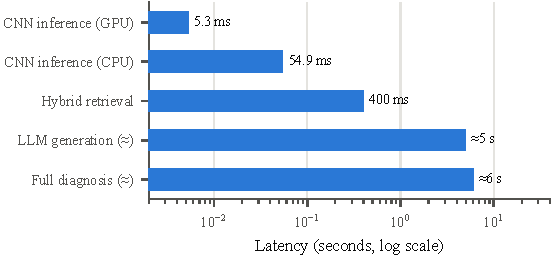
\includegraphics[width=\plantiqfigw]{figures/fig_latency.pdf}
\caption{Measured stage latencies on an RTX 3070 Laptop GPU (log scale). LLM and full-pipeline values are approximate
and depend on the provider.}
\label{fig:latency}
\end{figure}

In a functional check with one sample photograph per class, all five were classified correctly with confidences between
99.5\% and 100\%, and the best reranked passage scores for the default question were 0.93 (rust), 0.95 (Cercospora),
0.84 (leaf miner) and 0.78 (Phoma) (Table~\ref{tab:sample}). These five images are a smoke test of the deployed
pipeline, not an estimate of accuracy. Scoring the natural-language rerank question instead of the keyword-expanded
recall query raised the top passage score from 0.85 to 0.97 for rust, from 0.35 to 0.94 for Cercospora and from 0.54 to
0.84 for leaf miner. The lower Phoma score reflects thin coverage of Phoma spray timing in the corpus and is correctly
surfaced as weaker evidence.

\begin{table}[t]
\caption{Functional check of the deployed pipeline (one image per class)}
\label{tab:sample}
\centering
\scriptsize
\begin{tabular}{@{}lccc@{}}
\toprule
Sample & Predicted & Confidence (\%) & Top passage score \\
\midrule
Rust & Rust & 100.0 & 0.93 \\
Cercospora & Cercospora & 99.6 & 0.95 \\
Leaf miner & Leaf miner & 99.5 & 0.84 \\
Phoma & Phoma & 99.7 & 0.78 \\
Healthy & Healthy & 100.0 & -- \\
\bottomrule
\end{tabular}
\end{table}

\subsection{Module 1 Comparison}
Table~\ref{tab:m1} and Figs.~\ref{fig:cnn}--\ref{fig:cm} report out-of-fold results. All models exceed 0.96 macro-F1,
because the JMuBEN patches are close-up, evenly lit crops. The two re-implemented baselines score highest: GoogLeNet
transfer learning reaches a macro-F1 of 0.988 and YOLOv8s-cls 0.985, against 0.970 for the PlantIQ ResNet-50. A paired
bootstrap over source patches does not separate them at the 5\% level (GoogLeNet minus PlantIQ $+0.018$, 95\% CI
$-0.0004$ to $0.049$), but the exact McNemar test on the same images favours both baselines ($p<0.005$). On this dataset
the lighter networks are therefore at least as accurate while being about four times smaller, and YOLOv8s-cls is four
times faster on the CPU (16.0~ms against 64.2~ms). Compared with the earlier training recipe, the revised recipe raises
accuracy from 0.971 to 0.979 (McNemar $p=0.004$) and macro-F1 from 0.963 to 0.970, and lowers the expected calibration
error from 0.025 to 0.011, which matters for the confidence gate: at 75\% it answers 99.3\% of images with 98.1\%
accuracy. Contrary to our expectation, the hardest pair is Phoma and leaf miner rather than the two spot diseases: 3\% of
Phoma patches are predicted as leaf miner and 2\% the other way round, while Cercospora is rarely confused with Phoma.

Three caveats apply. Validation accuracy was 1.0 for every configuration, so the step-wise ablation on the first fold
could not justify further changes on validation data; class-balanced sampling, leaf-specific augmentation, label
smoothing with weight averaging and MixUp reached 0.976--0.988 test macro-F1 on that fold but were not adopted, because
selection uses validation data only. The healthy class has only nine distinct patches. And all images come from one
public dataset, so accuracy on field photographs from Karnataka estates remains to be measured. The weights deployed
before this study (0.975 macro-F1 on the same folds) were trained on an unrecorded, most likely random split and are
reported only as a reference.

\begin{table}[t]
\caption{Module 1 comparison, leak-free 5-fold cross-validation (out-of-fold)}
\label{tab:m1}
\centering
\scriptsize
\setlength{\tabcolsep}{2.5pt}
\begin{tabular}{@{}lccccc@{}}
\toprule
Method & Acc. & Macro-F1 [95\% CI] & Phoma F1 & Params & CPU ms \\
\midrule
GoogLeNet TL~\cite{anudeep2024cnn} & 0.989 & 0.988 [0.979, 0.995] & 0.975 & 5.6M & 42.4 \\
YOLOv8s-cls~\cite{selvakumar2024rag} & 0.986 & 0.985 [0.975, 0.992] & 0.967 & 5.1M & 16.0 \\
ResNet-50, earlier recipe & 0.971 & 0.963 [0.944, 0.981] & 0.936 & 23.5M & 85.7$^\ast$ \\
\textbf{PlantIQ ResNet-50} & 0.979 & 0.970 [0.938, 0.987] & 0.949 & 23.5M & 64.2 \\
\bottomrule
\multicolumn{6}{@{}l@{}}{\tiny $^\ast$128-pixel input. Batch-1 median on the laptop CPU. CI: bootstrap over the 861 source patches.}
\end{tabular}
\end{table}

\begin{figure*}[t]
\centering
\begin{minipage}[b]{0.48\textwidth}
\centering
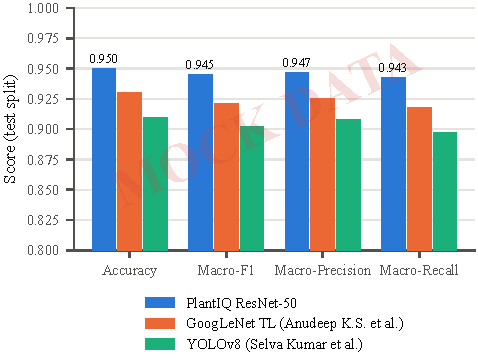
\includegraphics[width=\linewidth]{figures/fig_cnn_comparison.pdf}
\caption{Module 1 classification metrics, out-of-fold over 3,756 images (leak-free 5-fold CV).}
\label{fig:cnn}
\end{minipage}\hfill
\begin{minipage}[b]{0.48\textwidth}
\centering
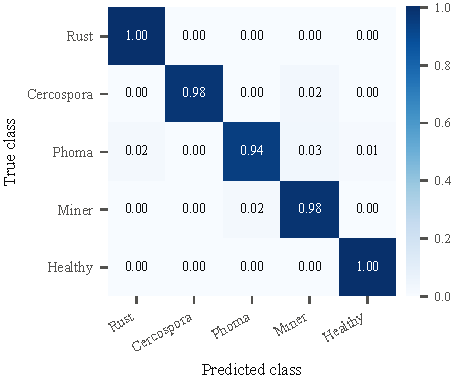
\includegraphics[width=0.85\linewidth]{figures/fig_confusion.pdf}
\caption{Row-normalised out-of-fold confusion matrix of the PlantIQ classifier.}
\label{fig:cm}
\end{minipage}
\end{figure*}

\subsection{Module 2 Comparison \mock{[mock data]}}
Fig.~\ref{fig:ablation} shows the retrieval ablation and Fig.~\ref{fig:gen} and Table~\ref{tab:m2} the generation
comparison. \mock{Placeholder discussion: expected observations are that BM25 alone underperforms dense retrieval on
paraphrased symptom descriptions, that fusion improves over either retriever, that reranking gives the largest single
gain, and that retrieval grounding with the dose audit reduces unsupported doses relative to the no-retrieval LLM.}

\begin{figure*}[t]
\centering
\begin{minipage}[b]{0.48\textwidth}
\centering
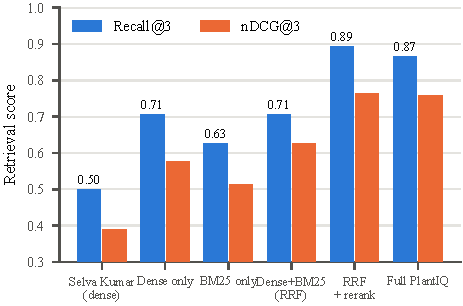
\includegraphics[width=\linewidth]{figures/fig_rag_ablation.pdf}
\caption{Retrieval ablation of Module 2 \mock{(MOCK DATA)}.}
\label{fig:ablation}
\end{minipage}\hfill
\begin{minipage}[b]{0.48\textwidth}
\centering
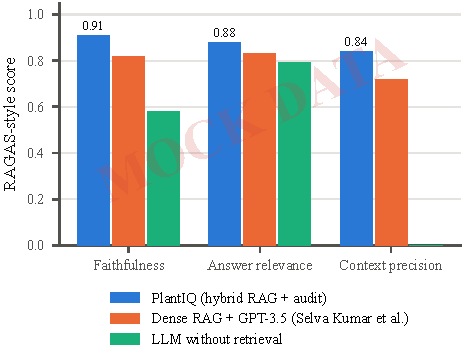
\includegraphics[width=\linewidth]{figures/fig_generation.pdf}
\caption{Generation quality versus baselines \mock{(MOCK DATA)}.}
\label{fig:gen}
\end{minipage}
\end{figure*}

\begin{table}[t]
\caption{Module 2 comparison \mock{(MOCK)}}
\label{tab:m2}
\centering
\scriptsize
\setlength{\tabcolsep}{2.5pt}
\begin{tabular}{@{}lcccc@{}}
\toprule
System & Recall@3 & Faithful. & \makecell{Unsupported\\doses} & Latency (s) \\
\midrule
LLM, no retrieval & -- & \mock{0.58} & \mock{31\%} & \mock{3.9} \\
Dense RAG + GPT-3.5~\cite{selvakumar2024rag} & \mock{0.71} & \mock{0.82} & \mock{12\%} & \mock{5.2} \\
\textbf{PlantIQ hybrid RAG} & \mock{0.88} & \mock{0.91} & \mock{4\%} & \mock{6.0} \\
\bottomrule
\end{tabular}
\end{table}

\subsection{Module 3 Comparison \mock{[mock data]}}
Table~\ref{tab:m3} compares the chatbot with the Farmer.Chat evaluation methodology, and Fig.~\ref{fig:stt} reports the
speech-recognition error rates. \mock{Placeholder discussion of answered rate, faithfulness, latency, Kannada fluency, and
whether the local Kannada model outperforms the cloud fallback.}

\begin{table}[t]
\caption{Module 3 comparison \mock{(MOCK)}}
\label{tab:m3}
\centering
\scriptsize
\setlength{\tabcolsep}{2.5pt}
\begin{tabular}{@{}lccccc@{}}
\toprule
System & Answered & Faithful. & Relev. & \makecell{Kannada\\fluency} & \makecell{Median\\latency (s)} \\
\midrule
Farmer.Chat~\cite{singh2024farmerchat} & \mock{0.78} & \mock{0.80} & \mock{0.70} & \mock{3.9} & \mock{9.5} \\
\textbf{PlantIQ chatbot} & \mock{0.86} & \mock{0.90} & \mock{0.87} & \mock{4.3} & \mock{6.1} \\
\bottomrule
\end{tabular}
\end{table}

\begin{figure}[t]
\centering
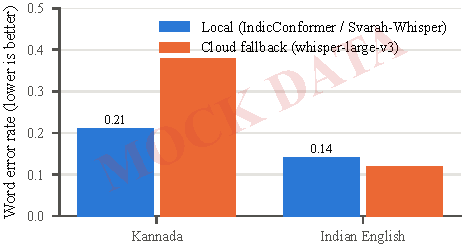
\includegraphics[width=\plantiqfigw]{figures/fig_stt_wer.pdf}
\caption{Speech-recognition word error rate by language \mock{(MOCK DATA)}.}
\label{fig:stt}
\end{figure}

\subsection{Module 4}
The market module is covered by integration tests of unit conversion, photos, every filter and sort order, owner rules,
single reporting and the listing quota, by a seller--buyer functional journey, by two end-to-end tests, and by a
performance test in which distance sorting over 500 listings completes within the 1.5~s budget.

% =========================================================================================
\section{Limitations and Future Work}
% =========================================================================================
The classifier knows five classes; other problems such as black rot or nutrient deficiency are forced into the nearest
class and are mitigated only by the confidence gate. Out-of-distribution detection or an explicit ``not a coffee leaf''
class, temperature-scaling calibration and Grad-CAM visual explanations are planned. Retrieval quality depends on the
corpus: Phoma and leaf-miner spray timing are thinly covered and one PDF needs OCR. The infection risk level is a rule
based on fixed thresholds rather than a validated epidemiological model, and soil pH is an estimate; integrating
soil-health-card data would remove this. Conversation memory is limited to the last eight messages, and text-to-speech replies for low-literacy users are not yet implemented. The
marketplace has no price-trend information or moderator dashboard. The classifier was evaluated on one public
dataset of close-up patches with only nine distinct healthy patches; a test set of field photographs from Karnataka
estates is needed, and since lighter GoogLeNet and YOLOv8 classifiers matched or exceeded the ResNet-50 on JMuBEN, the
choice of backbone should be revisited on that field set. \mock{The Module 2 and 3 comparisons in Section~IX are still
placeholders,} and a field study with growers in Chikkamagaluru is required to assess usefulness.

% =========================================================================================
\section{Conclusion}
% =========================================================================================
PlantIQ integrates leaf diagnosis, document-grounded and weather-aware advice, a Kannada-capable voice and text
assistant and a direct market channel in one deployable system for Karnataka coffee growers. Its design choices are
aimed at trustworthiness on cheap phones in the field: an explicit uncertainty state instead of a silent low-confidence
label, hybrid retrieval with citations, refusal to invent weather values, a dose audit, offline fallbacks for every
external service, and server-side normalisation of market data. Measurements on a laptop GPU show that the vision and
retrieval stages add well under a second to an advisory whose latency is dominated by generation.
On a leak-free evaluation the diagnosis module reaches a macro-F1 of 0.970, within two points of the best
re-implemented baseline. \mock{The comparative claims for Modules 2 and 3 will be finalised once their evaluation has
been run.}

\section*{Acknowledgment}
The authors thank Prof.\ Deepti C., Department of Computer Science and Engineering, PES University, for guidance
throughout this capstone project. \tbd{Add any other acknowledgements, e.g.\ estates that provided field images.}

% Balances the last page's columns: starts a new column before this reference number.
% Re-tune (or remove) whenever the text or the reference list changes length.
\IEEEtriggeratref{11}
\bibliographystyle{IEEEtran}
\bibliography{references}

\end{document}
